\begin{frame}{Các bước trong đường ống dữ liệu Pháp Điển}

\begin{figure}[H]
\centering
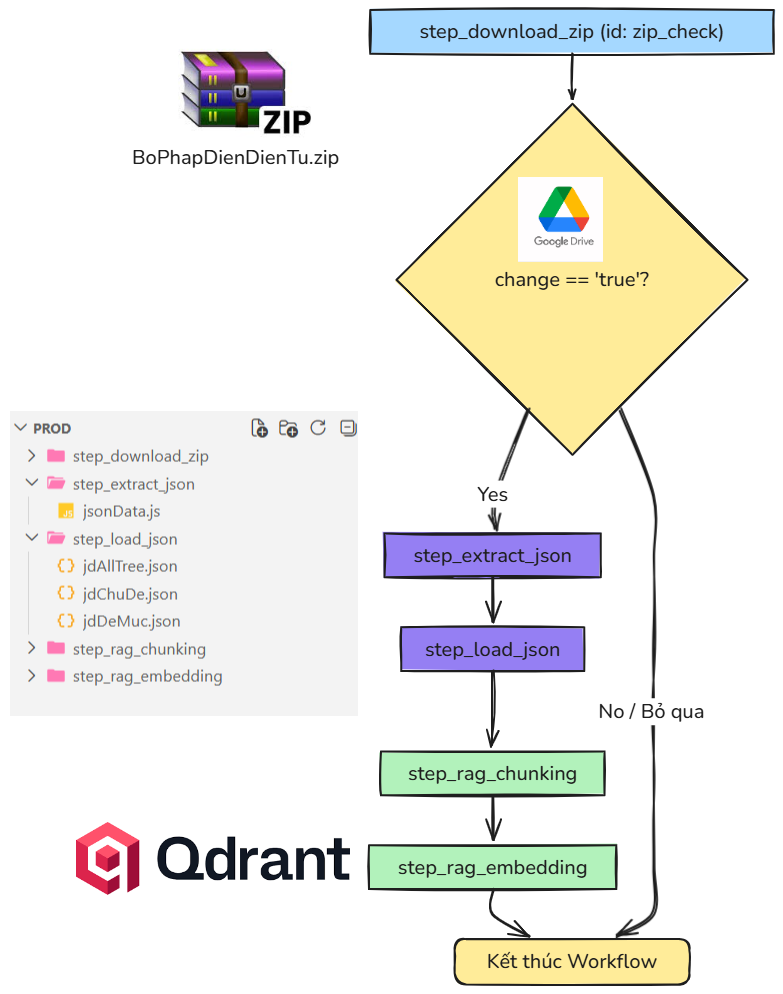
\includegraphics[height=0.7\textheight,width=0.9\textwidth,keepaspectratio]{pictures/step3.excalidraw.png}
\caption{Sơ đồ các bước thực hiện của đường ống dữ liệu Pháp Điển}
\end{figure}

\note{
Sơ đồ mô tả quy trình từng bước của đường ống dữ liệu Pháp Điển.
Quy trình bắt đầu từ việc tải file ZIP tự động (\texttt{step\_download\_zip}), tính toán mã băm MD5 để kiểm tra sự thay đổi dữ liệu so với phiên bản trước, giải nén và trích xuất cấu trúc đề mục ra các file JSON riêng biệt, sau đó chạy các tác vụ phân tích cấu trúc và lưu kết quả vector hóa.
}
\end{frame}
